\tikzset{every picture/.style={line width=0.75pt}} %set default line width to 0.75pt        

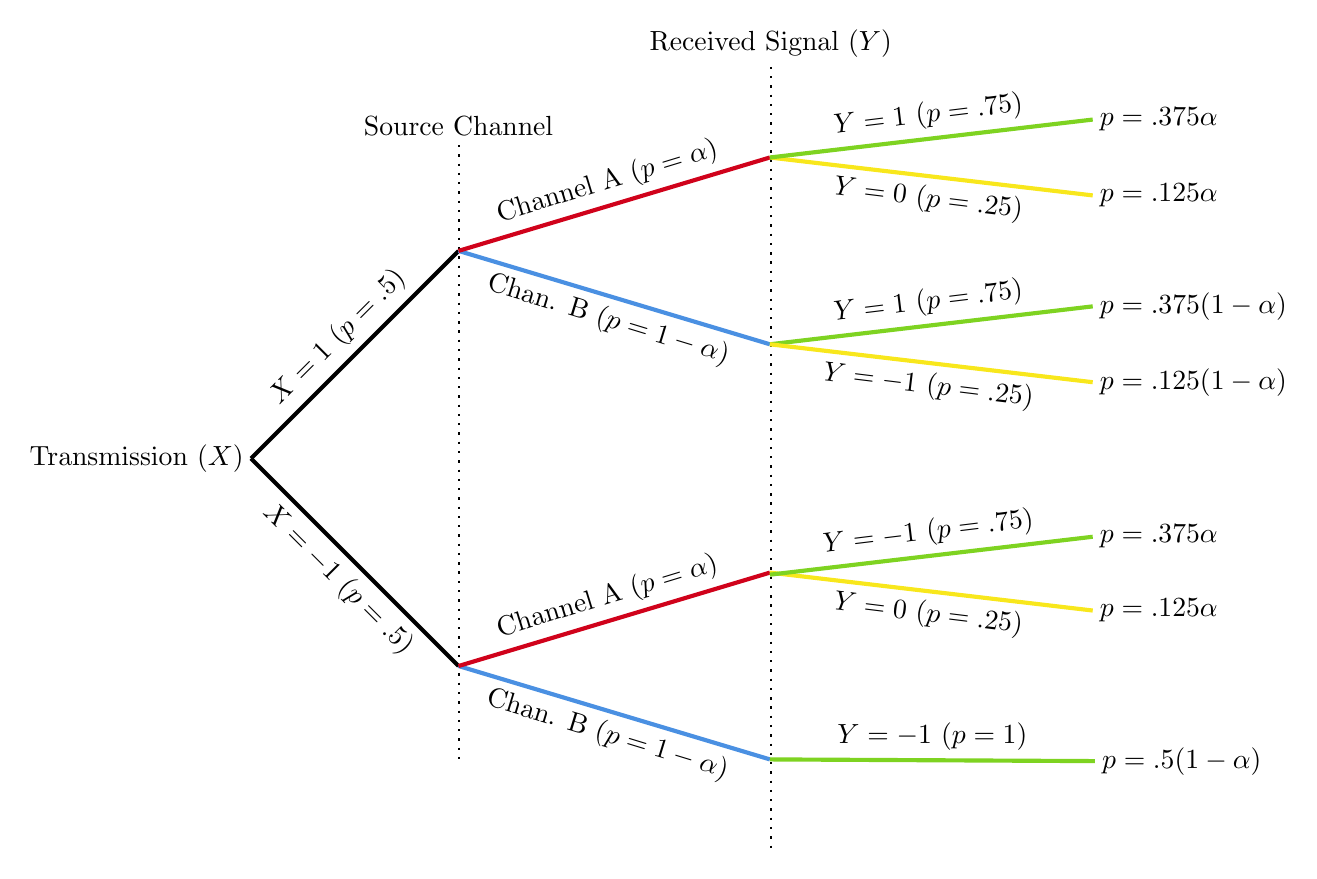
\begin{tikzpicture}[x=0.75pt,y=0.75pt,yscale=-1,xscale=1]
%uncomment if require: \path (0,493); %set diagram left start at 0, and has height of 493

%Straight Lines [id:da23791128150940755] 
\draw [line width=1.5]    (124,251) -- (224,151) ;
%Straight Lines [id:da3966057563521548] 
\draw [line width=1.5]    (124,251) -- (224,351) ;
%Straight Lines [id:da915484597228999] 
\draw  [dash pattern={on 0.84pt off 2.51pt}]  (224,100) -- (224,396.42) ;
%Straight Lines [id:da1241748882024809] 
\draw [color={rgb, 255:red, 74; green, 144; blue, 226 }  ,draw opacity=1 ][line width=1.5]    (224,151) -- (374,196) ;
%Straight Lines [id:da5569456827980495] 
\draw [color={rgb, 255:red, 208; green, 2; blue, 27 }  ,draw opacity=1 ][line width=1.5]    (374,106) -- (224,151) ;
%Straight Lines [id:da011409041725653823] 
\draw [color={rgb, 255:red, 74; green, 144; blue, 226 }  ,draw opacity=1 ][line width=1.5]    (224,351) -- (374,396) ;
%Straight Lines [id:da8043679678690399] 
\draw [color={rgb, 255:red, 208; green, 2; blue, 27 }  ,draw opacity=1 ][line width=1.5]    (374,306) -- (224,351) ;
%Straight Lines [id:da9802980049289851] 
\draw  [dash pattern={on 0.84pt off 2.51pt}]  (374.42,62.29) -- (374.42,439.71) ;
%Straight Lines [id:da4884123484523494] 
\draw [color={rgb, 255:red, 248; green, 231; blue, 28 }  ,draw opacity=1 ][line width=1.5]    (374,106) -- (529.54,124.27) ;
%Straight Lines [id:da12971510506081663] 
\draw [color={rgb, 255:red, 126; green, 211; blue, 33 }  ,draw opacity=1 ][line width=1.5]    (529.54,177.73) -- (374,196) ;
%Straight Lines [id:da7130390548310087] 
\draw [color={rgb, 255:red, 126; green, 211; blue, 33 }  ,draw opacity=1 ][line width=1.5]    (529.54,87.73) -- (374,106) ;
%Straight Lines [id:da7886014049297126] 
\draw [color={rgb, 255:red, 248; green, 231; blue, 28 }  ,draw opacity=1 ][line width=1.5]    (374,196) -- (529.54,214.27) ;
%Straight Lines [id:da8437771671847172] 
\draw [color={rgb, 255:red, 248; green, 231; blue, 28 }  ,draw opacity=1 ][line width=1.5]    (374,306) -- (529.54,324.27) ;
%Straight Lines [id:da4450873514693551] 
\draw [color={rgb, 255:red, 126; green, 211; blue, 33 }  ,draw opacity=1 ][line width=1.5]    (529.54,288.73) -- (374,307) ;
%Straight Lines [id:da04003805736905319] 
\draw [color={rgb, 255:red, 126; green, 211; blue, 33 }  ,draw opacity=1 ][line width=1.5]    (530.6,396.82) -- (374,396) ;

% Text Node
\draw (171.6,198.6) node [anchor=south] [inner sep=0.75pt]  [rotate=-315]  {$X=1\ ( p=.5)$};
% Text Node
\draw (171.6,303.4) node [anchor=north] [inner sep=0.75pt]  [rotate=-45]  {$X=-1\ ( p=.5)$};
% Text Node
\draw (122,251) node [anchor=east] [inner sep=0.75pt]   [align=left] {Transmission ($\displaystyle X$)};
% Text Node
\draw (224,97) node [anchor=south] [inner sep=0.75pt]   [align=left] {Source Channel};
% Text Node
\draw (298.12,125.63) node [anchor=south] [inner sep=0.75pt]  [rotate=-343] [align=left] {Channel A ($\displaystyle p=\alpha $)};
% Text Node
\draw (298.54,176.49) node [anchor=north] [inner sep=0.75pt]  [rotate=-17] [align=left] {Chan. B ($\displaystyle p=1-\alpha $)};
% Text Node
\draw (298.12,325.63) node [anchor=south] [inner sep=0.75pt]  [rotate=-343] [align=left] {Channel A ($\displaystyle p=\alpha $)};
% Text Node
\draw (298.12,376.37) node [anchor=north] [inner sep=0.75pt]  [rotate=-17] [align=left] {Chan. B ($\displaystyle p=1-\alpha $)};
% Text Node
\draw (374.42,59.29) node [anchor=south] [inner sep=0.75pt]   [align=left] {Received Signal ($\displaystyle Y$)};
% Text Node
\draw (451.4,118.11) node [anchor=north] [inner sep=0.75pt]  [rotate=-7] [align=left] {$\displaystyle Y=0\ ( p=.25)$};
% Text Node
\draw (451.4,183.89) node [anchor=south] [inner sep=0.75pt]  [rotate=-353] [align=left] {$\displaystyle Y=1\ ( p=.75)$};
% Text Node
\draw (451.4,93.89) node [anchor=south] [inner sep=0.75pt]  [rotate=-353] [align=left] {$\displaystyle Y=1\ ( p=.75)$};
% Text Node
\draw (451.4,208.11) node [anchor=north] [inner sep=0.75pt]  [rotate=-7] [align=left] {$\displaystyle Y=-1\ ( p=.25)$};
% Text Node
\draw (451.4,318.11) node [anchor=north] [inner sep=0.75pt]  [rotate=-7] [align=left] {$\displaystyle Y=0\ ( p=.25)$};
% Text Node
\draw (451.4,294.89) node [anchor=south] [inner sep=0.75pt]  [rotate=-353] [align=left] {$\displaystyle Y=-1\ ( p=.75)$};
% Text Node
\draw (452.3,393.41) node [anchor=south] [inner sep=0.75pt]   [align=left] {$\displaystyle Y=-1\ ( p=1)$};
% Text Node
\draw (531.54,87.73) node [anchor=west] [inner sep=0.75pt]    {$p=.375\alpha $};
% Text Node
\draw (531.54,124.27) node [anchor=west] [inner sep=0.75pt]    {$p=.125\alpha $};
% Text Node
\draw (531.54,177.73) node [anchor=west] [inner sep=0.75pt]    {$p=.375( 1-\alpha )$};
% Text Node
\draw (531.54,214.27) node [anchor=west] [inner sep=0.75pt]    {$p=.125( 1-\alpha )$};
% Text Node
\draw (531.54,288.73) node [anchor=west] [inner sep=0.75pt]    {$p=.375\alpha $};
% Text Node
\draw (531.54,324.27) node [anchor=west] [inner sep=0.75pt]    {$p=.125\alpha $};
% Text Node
\draw (532.6,396.82) node [anchor=west] [inner sep=0.75pt]    {$p=.5( 1-\alpha )$};


\end{tikzpicture}
